\documentclass[a4paper,12pt]{article}
\usepackage{ctex}
\usepackage{amsmath}
\usepackage{graphicx}
\usepackage{geometry}
\usepackage{multirow}
\usepackage{float}
\usepackage{subcaption}
\usepackage{csvsimple}
\geometry{left=2.5cm,right=2.5cm,top=2.5cm,bottom=2.5cm}
\graphicspath{{figures/}{results/}}
\begin{document}
\begin{titlepage}
    \centering
    \vfill
    {\zihao{0}\bfseries 电子测试与实验技术\\[0.6em]实验报告\par}
    \vfill
    \vfill

    \begin{minipage}{0.72\textwidth}
        \zihao{-2}
        学\quad\quad 院：\underline{\makebox[7.5cm][l]{光学与电子信息学院}}\\[1.6em]
        班\quad\quad 级：\underline{\makebox[7.5cm][l]{光电信息科学与工程202409班}}\\[1.6em]
        姓\quad\quad 名：\underline{\makebox[7.5cm][l]{陈\quad 恪\quad 瑾}}\\[1.6em]
        学\quad\quad 号：\underline{\makebox[7.5cm][l]{U 2 0 2 4 1 3 9 2 5}}\\[1.6em]
        实验时间：\underline{\makebox[7.5cm][l]{2026 年 04 月 09 日}}
    \end{minipage}

    \vfill
    \vfill
\end{titlepage}

\setcounter{page}{1}



\section*{一、实验名称}
单级共射放大电路。

\section*{二、实验目的}
\begin{enumerate}
    \item 掌握晶体管放大电路静态工作点设置与调整方法。
    \item 了解电路参数变化对静态工作点的影响。
    \item 掌握晶体管放大电路的安装与调试技术。
    \item 掌握晶体管放大电路性能指标（Av、BW）的测试方法。
    \item 了解负反馈对放大电路性能的影响。
    
\end{enumerate}

\section*{三、实验元器件}
\begin{table}[H]
    \centering
    \begin{tabular}{|c|c|c|}
        \hline
        类型 & 型号（参数） & 数量/单位 \\
        \hline
        三极管 & 9018 & 1/只 \\
        \hline
        电位器 & 100\,k$\Omega$ & 1/只 \\
        \hline
        \multirow{5}{*}{电阻} & 51\,$\Omega$ & 1/只 \\
        \cline{2-3}
         & 1\,k$\Omega$ & 1/只 \\
        \cline{2-3}
         & 5.1\,k$\Omega$ & 2/只 \\
        \cline{2-3}
         & 10\,k$\Omega$ & 2/只 \\
        \cline{2-3}
         & 100\,k$\Omega$ & 1/只 \\
        \hline
        \multirow{2}{*}{电容} & 10\,$\mu$F & 2/只 \\
        \cline{2-3}
         & 47\,$\mu$F & 1/只 \\
        \hline
    \end{tabular}
    \caption{实验元器件清单}
\end{table}



\section*{四、实验原理}
\subsection*{4.1 参考电路}
该实验采用自动稳定静态工作点的分压式射极偏置共射放大电路，具有较好的温度稳定性。三极管选用 SS9018，电位器 $R_p$ 用于调节静态工作点。


\begin{figure}[H]
    \centering
    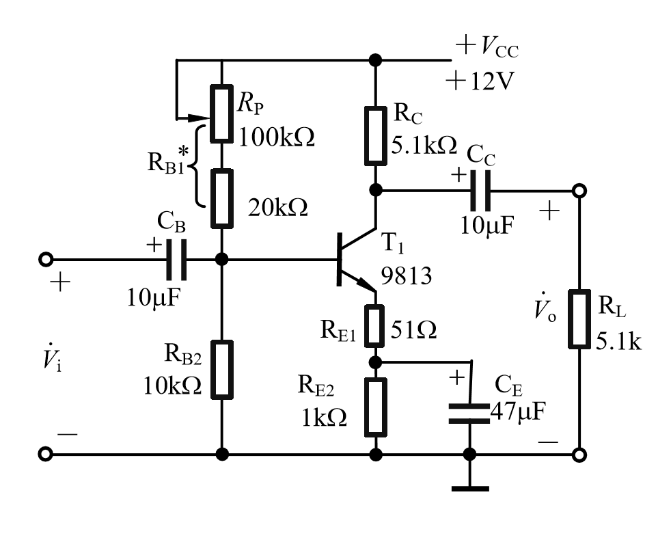
\includegraphics[width=0.72\textwidth]{ExperimentalReferenceCircuit.png}
    \caption{实验参考电路}
    \label{fig:ce_reference}
\end{figure}

\subsection*{4.2 静态工作点的估算与调整}
静态工作点是指输入交流信号为 0 时三极管的基极电流 $I_{BQ}$、集电极电流 $I_{CQ}$ 和集电极-发射极电压 $V_{CEQ}$。为获得尽可能大的不失真输出，静态工作点通常应选在交流负载线中点附近。工作点偏高易产生饱和失真，偏低易产生截止失真。

\begin{figure}[H]
    \centering
    \begin{subfigure}{0.47\textwidth}
        \centering
        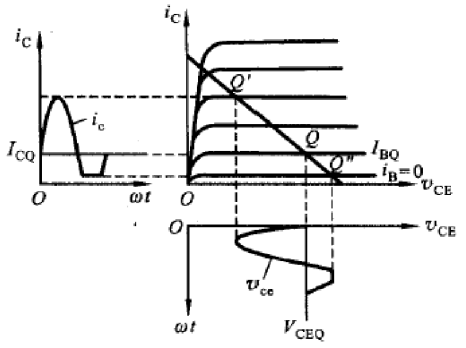
\includegraphics[width=\textwidth]{WaveformofCutoffDistortion.png}
        \caption{截止失真波形}
        \label{fig:cutoff_distortion}
    \end{subfigure}
    \hfill
    \begin{subfigure}{0.47\textwidth}
        \centering
        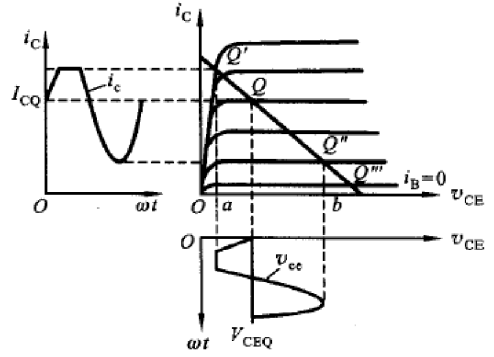
\includegraphics[width=\textwidth]{SaturationDistortionWaveform.png}
        \caption{饱和失真波形}
        \label{fig:saturation_distortion}
    \end{subfigure}
    \caption{非线性失真波形示意}
    \label{fig:nonlinear_distortion}
\end{figure}

提取参考电路的直流通路可得：

\begin{figure}[H]
    \centering
    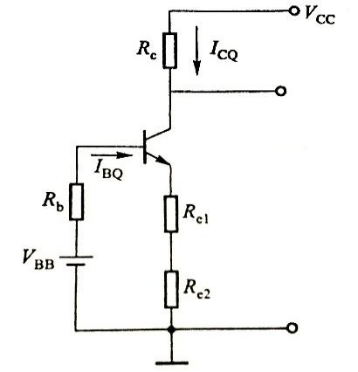
\includegraphics[width=0.62\textwidth]{EquivalentCircuit.png}
    \caption{直流等效通路}
    \label{fig:dc_equivalent}
\end{figure}

其中
\[
R_B = R_{B11} \parallel R_{B12}.
\]
开路电压
\[
V_{BB} = \frac{R_{B12}}{R_{B11}+R_{B12}}V_{CC}.
\]
静态工作点近似计算式为
\[
I_{BQ} = \frac{V_{BB}-V_{BEQ}}{R_B+(1+\beta)(R_{E1}+R_{E2})},
\]
\[
I_{CQ} = \beta I_{BQ},
\]
\[
V_{CEQ} \approx V_{CC}-(R_C+R_{E1}+R_{E2})I_{CQ}.
\]
由上式可见，静态工作点与电路参数及三极管 $\beta$ 有关；当其他参数固定时，可通过调节 $R_p$ 改变工作点。$R_p$ 调小，工作点升高；$R_p$ 调大，工作点降低。

\subsection*{4.3 电压增益的测量}
测量电压增益、输入电阻和输出电阻等指标时，应保证放大器在线性工作区且工作于中频段。电压增益定义为
\[
A_v = \frac{V_o}{V_i} \approx -\frac{\beta\,(R_C\parallel R_L)}{r_{be}+(1+\beta)R_{E1}}.
\]

\subsection*{4.4 输入电阻的测量}
输入电阻 $R_i$ 表征放大电路对信号源的负载作用。$R_i$ 越大，对前级影响越小。该电路中可近似写为
\[
R_i = R_{B11}\parallel R_{B12}\parallel \left[r_{be}+(1+\beta)R_{E1}\right].
\]
三极管小信号输入电阻可近似为
\[
r_{be} \approx 200 + (1+\beta)\frac{26\,\mathrm{mV}}{I_{CQ}(\mathrm{mA})}.
\]

\subsection*{4.5 输出电阻的测量}
输出电阻 $R_o$ 表征电路带负载能力，$R_o$ 越小，带负载能力越强。对本实验电路，在忽略晶体管输出电阻影响时，可近似取
\[
R_o \approx R_C.
\]

\subsection*{4.6 注意事项}
\begin{enumerate}
    \item 组装电路时，不要弯曲三极管三个电极，建议垂直插入面包板孔位。
    \item 组装完成后，先调好稳压电源并检查无误，再接入电路并上电。
    \item 测试静态工作点时，应使输入信号 $V_i=0$。
    \item 本实验元器件和连接点较多，需重点检查接触可靠性，避免接触不良导致故障。
    \item 由于信号源存在内阻且放大电路输入电阻有限，测量 $V_i$ 时应在电路连接完成后进行，以减小测量误差。
\end{enumerate}

\section*{五、硬件实验内容}
\subsection*{5.1 调整静态工作点}
\begin{enumerate}
    \item 输入正弦信号，设定 $f=1\,\mathrm{kHz}$、$V_{i,pp}=100\,\mathrm{mV}$。
    \item 缓慢增大输入幅值，观察先出现截止失真还是饱和失真（本电路为 NPN 三极管共射反相放大）。
    \item 若先出现饱和失真，说明静态工作点偏高，应适当增大电位器 $R_p$ 使工作点下移；若先出现截止失真，说明静态工作点偏低，应适当减小 $R_p$ 使工作点上移。
    \item 重复调节，直至增大输入时饱和失真与截止失真近似同时出现；再微调输入幅值至输出刚好不失真，完成静态工作点调整。
\end{enumerate}


\subsection*{5.2 静态工作点测量}
\begin{enumerate}
    \item 静态工作点调好后，去掉输入正弦信号。
    \item 用万用表 hFE 档测量三极管直流电流放大倍数 $\beta$。
    \item 测量三极管基极、射极、集极静态电压，分别记为 $V_{BQ}$、$V_{EQ}$、$V_{CQ}$。
    \item 测量此时电位器接入电路的阻值 $R_p$。
    \item 将测量数据代入公式，计算 $V_{CEQ}$、$I_{CQ}$ 与 $I_{BQ}$。
\end{enumerate}

\subsection*{5.3 电压放大倍数测量}
\begin{enumerate}
    \item 在输出波形不失真的条件下，同时测量输入与输出电压波形。
    \item 读取峰峰值或有效值，按
          \[
          A_v=\frac{V_o}{V_i}
          \]
          计算电压增益。
\end{enumerate}

\subsection*{5.4 幅频响应特性曲线测量}
\begin{enumerate}
    \item 先在中频段（$f=1\,\mathrm{kHz}$）测得中频电压增益 $A_{vm}$。
    \item 计算三分贝点对应增益：$A_{vL}=A_{vH}=0.707A_{vm}$，并据此确定目标输出幅值。
    \item 保持输入幅值不变，降低频率，直到输出降至目标值，记为下限频率 $f_L$。
    \item 保持输入幅值不变，提高频率，直到输出降至目标值，记为上限频率 $f_H$。
    \item 计算通频带：
          \[
          BW=f_H-f_L.
          \]
\end{enumerate}

\subsection*{5.5 测量输入电阻}
\begin{enumerate}
    \item 在信号源与放大电路输入端串联一个与输入阻抗接近的电阻（如 $3.3\,\mathrm{k}\Omega$ 或 $5.1\,\mathrm{k}\Omega$）。
    \item 测得信号源电压 $V_s$ 及输入端电压 $V_i$，代入实验公式$R_i = \frac{V_i}{V_s - V_i}R$计算输入电阻 $R_i$。
\end{enumerate}八、实验分析与数据处理

\subsection*{5.6 测量输出电阻}
\begin{enumerate}
    \item 测量接负载时负载电阻上的输出电压 $V_{oL}$。
    \item 将负载开路后测量开路输出电压 $V_o$，代入实验公式$R_o = (\frac{V_o}{V_{oL}} - 1)R_L$计算输出电阻 $R_o$。
\end{enumerate}

\section*{六、EDA仿真实验内容}
\subsection*{6.1 测试静态工作点（Bias Point 分析）}
根据硬件实验中调整得到的静态工作点参数，仿真时将电位器等效为固定电阻
$R_p=28\,\mathrm{k}\Omega$，取三极管直流电流放大倍数 $\beta=85$，并去掉交流输入信号。
在该条件下进行 ``Bias Point'' 分析，得到静态工作点电压 $V_{BQ}$、$V_{EQ}$、$V_{CQ}$。

\subsection*{6.2 观测输入输出波形并计算电压放大倍数（瞬态分析）}
在输出波形不失真的条件下，测得输入与输出幅值，电压增益按
\[
A_v=\frac{V_o}{V_i}
\]
计算。设置输入信号为 $V_{i,pp}=60\,\mathrm{mV}$、$f=1\,\mathrm{kHz}$（中频），仿真得到
$V_{o,pp}=2.0299\,\mathrm{V}$，故
\[
A_v\approx\frac{2.0299}{0.060}=33.83.
\]

\subsection*{6.3 观测幅频响应与相频响应}
AC 分析结果表明：中频增益 $A_v=30.710$，上限频率 $f_H=13.965\,\mathrm{MHz}$，
下限频率 $f_L=52.462\,\mathrm{Hz}$，通频带
\[
BW=f_H-f_L\approx 13.965\,\mathrm{MHz}.
\]
相频响应曲线显示：当频率为中频 $f=25.864\,\mathrm{kHz}$ 时，相位差约为
$-180^\circ$，符合共射极反相放大的特性。

\subsection*{6.4 观测输入阻抗的频率响应}
在信号源与输入端之间串联 $5.1\,\mathrm{k}\Omega$ 电阻，进行 AC 仿真并绘制
\[
\left(\frac{V(V_i)}{V(V_s)-V(V_i)}\right)\times 5.1\,\mathrm{k}\Omega
\]
对应曲线，以观察输入阻抗的频率响应。由曲线可见，中频时输入阻抗约为
$3.26\,\mathrm{k}\Omega$。

\subsection*{6.5 观测输出阻抗的频率响应}
将输入信号源短路，并将负载电阻替换为小信号正弦源，测量输出端电压与电流比值，
绘制输出阻抗的频率响应曲线。由图可见，中频时输出阻抗约为
$4.98\,\mathrm{k}\Omega$。



\section*{七、硬件实验结果分析}
\subsection*{7.1 静态工作点测量数据}
\begin{table}[H]
    \centering
    \begin{tabular}{|c|c|c|c|c|c|}
        \hline
        $V_{BQ}$ & $V_{EQ}$ & $V_{CQ}$ & $I_c = \frac{V_cc - V_c}{R_{c1}}$ & $ V_{CEQ} = V_{CQ} - V_{EQ}$ \\
        \hline
        2.14350\,V & 1.43499\,V & 5.2384\,V & 1.3258\,mA & 3.80341 \, V\\
        \hline
    \end{tabular}
    \caption{静态工作点原始测量数据}
\end{table}

在本次实验的电路中，$R_{C1} = 5.1\,\mathrm{k}\Omega$，$V_{CC}=12\,\mathrm{V}$，代入上表数据计算得
\[I_{CQ} = \frac{V_{CC} - V_{CQ}}{R_{C1}} = \frac{12 - 5.2384}{5.1} = 1.3258\,\mathrm{mA},\]
\[V_{CEQ} = V_{CQ} - V_{EQ} = 5.2384 - 1.43499 = 3.80341\,\mathrm{V}.\]
整理为下表：

\begin{table}[H]
    \centering
    \begin{tabular}{|c|c|c|c|}
        \hline
        参数 & $I_{CQ}$ & $V_{CEQ}$  \\
        \hline
        数值 & 1.667\,mA & 1.745\,V  \\
        \hline
    \end{tabular}
    \caption{静态工作点计算结果}
\end{table}

根据实验讲义，一般 $V_{BQ}= (3 \textasciitilde 5)\,\mathrm{V}$，$V_{CEQ}$ 应为正的几伏。若 $V_{CEQ}\approx V_{CC}$，说明晶体管截止；若 $V_{CEQ}<0.5\,\mathrm{V}$，说明晶体管饱和。由上表中的测量结果可知，本实验中晶体管工作在放大区。

\subsection*{7.2 放大倍数计算数据}
将波形调整到最大不失真，示波器波形如图：
\begin{figure}[H]
    \centering
    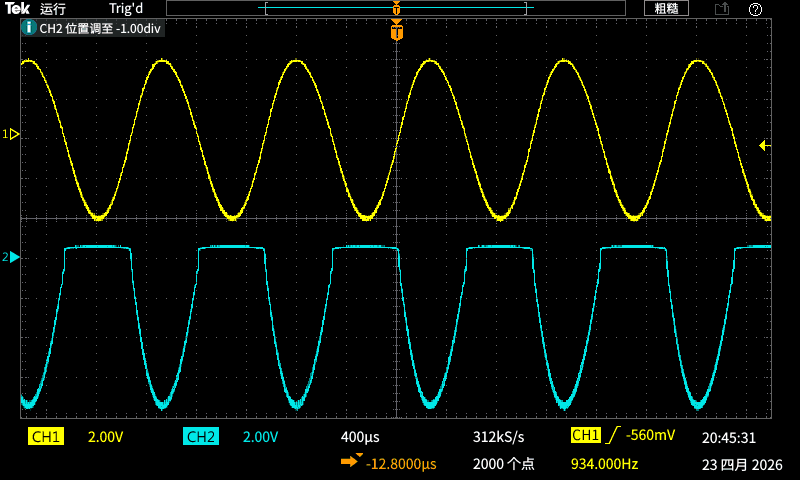
\includegraphics[width=0.72\textwidth]{figures/oscilloscope/figure2.PNG}
    \caption{最大不失真测量波形}
\end{figure}
测得输入峰峰值 $V_{ipp}=0.216\,\mathrm{V}$，输出峰峰值 $V_{opp}=6.72\,\mathrm{V}$，代入公式计算电压增益

\[
A_v = \frac{V_{ipp}}{V_{opp}} = \frac{6.72}{0.216}=31.11
\]

\subsection*{7.3 幅频响应特性曲线测量数据}
原始测量数据如下表：
\begin{table}[H]
    \centering
    \caption{幅频响应原始实验数据}
    \scriptsize
    \csvautotabular{figures/datas/BW/bw_sorted_with_av.csv}
\end{table}

\begin{figure}[H]
    \centering
    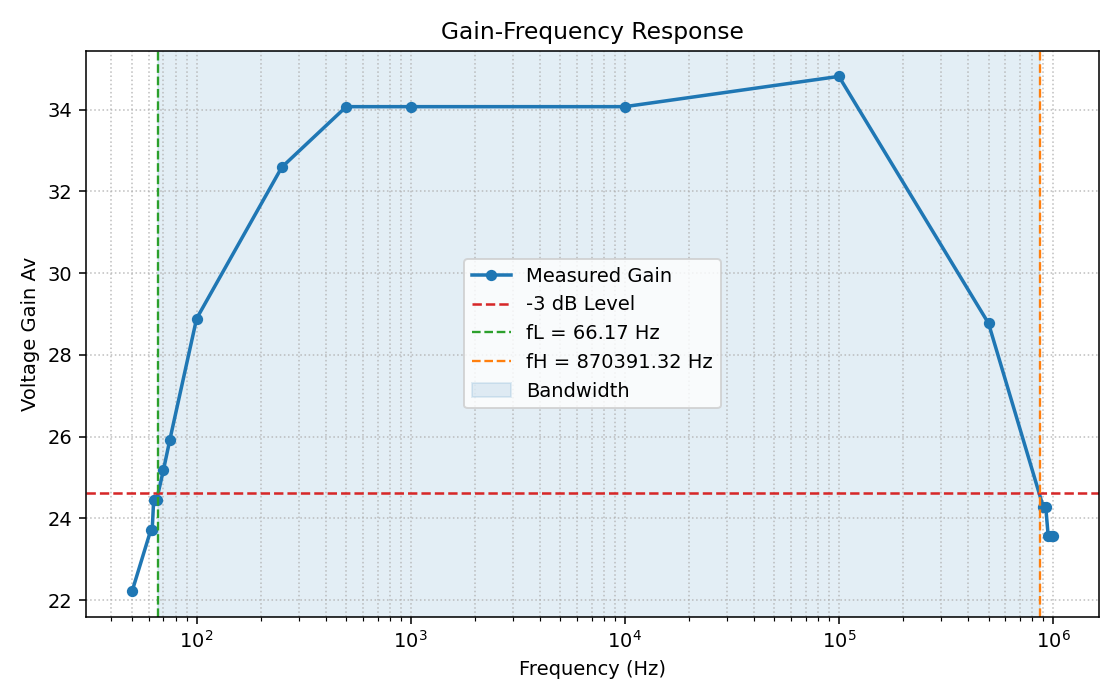
\includegraphics[width=0.78\textwidth]{figures/datas/BW/gain_frequency_bw.png}
    \caption{幅频响应曲线}
\end{figure}

计算得到最大电压增益
\[
A_{v,\max}=34.81,
\]
三分贝点增益
\[
A_{v,-3\mathrm{dB}}=\frac{A_{v,\max}}{\sqrt{2}}=24.62.
\]
根据数学分析计算可得下限频率与上限频率分别为
\[
f_L=66.17\,\mathrm{Hz},\qquad f_H=870.39\,\mathrm{kHz}.
\]
故通频带
\[
BW=f_H-f_L\approx 870.33\,\mathrm{kHz}.
\]
\begin{table}[H]
    \centering
    \begin{tabular}{|c|c|c|c|c|c|}
        \hline
         $A_{v,1kHz}$ & $A_{v,\max}$ &  $A_{v,-3\mathrm{dB}}$ &  $f_L$ &  $f_H$ &  $BW$ \\
        \hline
        34.074 &34.81 & 24.62 & 66.17\,Hz & 870.39\,kHz & 870.33\,kHz \\
        \hline
    \end{tabular}
    \caption{幅频响应特性计算结果}
\end{table}

分析：实测增益峰值大于 30，且低频端与高频端均出现明显下降，满足单级共射放大电路的幅频响应特征。

\subsection*{7.4 输入电阻测量数据}
先试用$5.1k\Omega$电阻测量，计算得到输入电阻约为$4.12k\Omega$，为了使串联电阻与输入电阻更为接近提高输入电阻测试准确度，改为使用$4.7k\Omega$电阻测量，测量数据如下表：
\begin{table}[H]
    \centering
    \begin{tabular}{|c|c|c|c|c|}
        \hline
        $V_s$ & $V_i$ & $R$ & $R_i$ \\
        \hline
        114\,mV & 54\,mV & 4.7\,k$\Omega$ & 4.29\,k$\Omega$ \\
        \hline
    \end{tabular}
    \caption{输入电阻测试数据}
    \end{table}
    根据输入电阻计算公式可得：
$$ R_i = \frac{V_i}{V_s - V_i } R = \frac{0.054}{0.114 - 0.054} \times 4.7\,\mathrm{k}\Omega = 4.29\,\mathrm{k}\Omega. $$


\subsection*{7.5 输出电阻测量数据}
根据实验原理连接电路并测量，测量数据如下表：
\begin{table}[H]
    \centering
    \begin{tabular}{|c|c|c|c|c|}
        \hline
        $V_o$ & $V_{oL}$ & $R_L$ & $R_o$ \\
        \hline
        7.00\,V & 3.80\,V & 5.1\,k$\Omega$ & 4.29\,k$\Omega$ \\
        \hline
    \end{tabular}
    \caption{输出电阻测试数据}
    \end{table}

根据输出电阻计算公式可得：
$$ R_o = \left( \frac{V_o}{V_{oL}} - 1 \right) R_L = \left( \frac{7.00}{3.80} - 1 \right) \times 5.1\,\mathrm{k}\Omega = 4.29\,\mathrm{k}\Omega. $$

\subsection*{7.6 饱和失真和截止失真测量}
\subsubsection*{7.6.1 饱和失真测量}
将滑动变阻器调至$0\,\Omega$，输入信号频率设为$1\,\mathrm{kHz}$，当输入峰峰值为$0.84\,\mathrm{V}$时，输出波形出现明显的饱和失真，如图所示：
\begin{figure}[H]
    \centering
    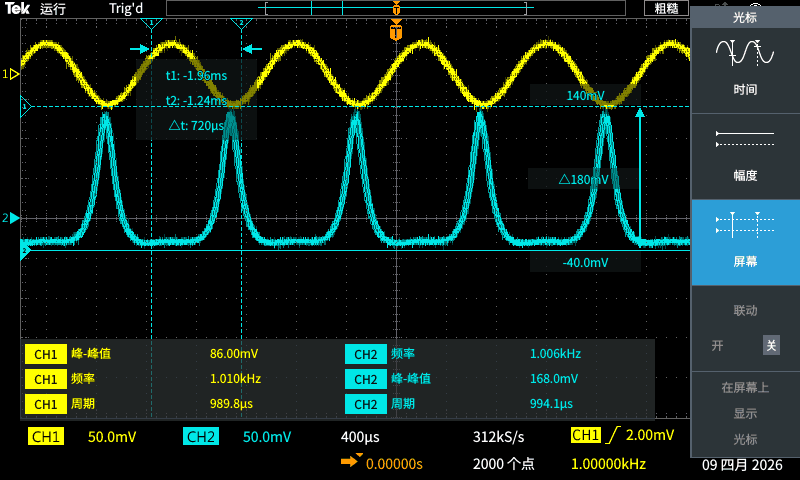
\includegraphics[width=0.72\textwidth]{figures/oscilloscope/figure6.PNG}
    \caption{饱和失真波形}
\end{figure}
对此时BJT的静态工作点测量，得到下表：
\begin{table}[H]
    \centering
    \begin{tabular}{|c|c|c|c|}
        \hline
        $V_{EQ}$ & $V_{BQ}$ & $V_{CQ}$ \\
        \hline
        2.3059\,V & 3.0535\,V & 2.3730\,V \\
        \hline
    \end{tabular}
    \caption{饱和失真测量数据}
\end{table}
\subsubsection*{7.6.2 截止失真测量}
将滑动变阻器调至$100\,\mathrm{k}\Omega$，输入信号频率设为$1\,\mathrm{kHz}$，当输入峰峰值为$1.10\,\mathrm{V}$时，输出波形出现明显的截止失真，如图所示：
\begin{figure}[H]
    \centering
    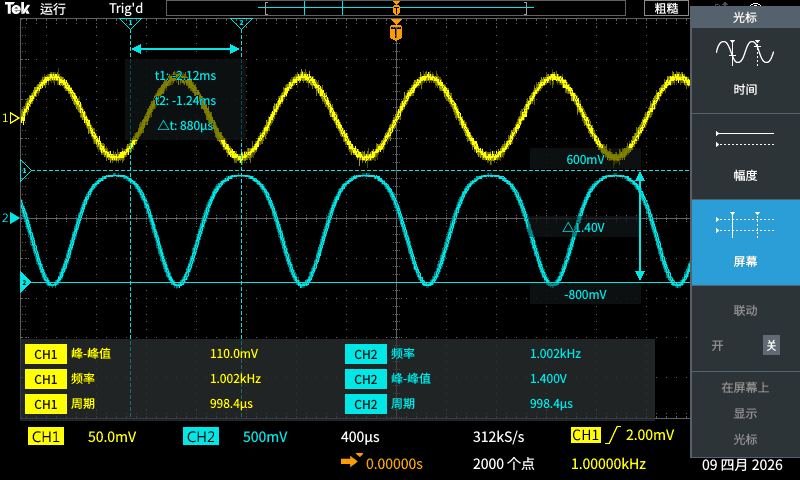
\includegraphics[width=0.72\textwidth]{figures/oscilloscope/figure5.PNG}
    \caption{截止失真波形}
\end{figure}
对此时BJT的静态工作点测量，得到下表：
\begin{table}[H]
    \centering
    \begin{tabular}{|c|c|c|c|}
        \hline
        $V_{EQ}$ & $V_{BQ}$ & $V_{CQ}$ \\
        \hline
        0.26584\,V & 0.91875\,V & 10.7524\,V \\
        \hline
    \end{tabular}
    \caption{截止失真测量数据}
\end{table}

\section*{八、EDA仿真实验结果分析}
根据原理图在Multisim中搭建仿真电路，如图所示，进行仿真分析并与硬件实验结果进行对比分析。
\begin{figure}[H]
    \centering
    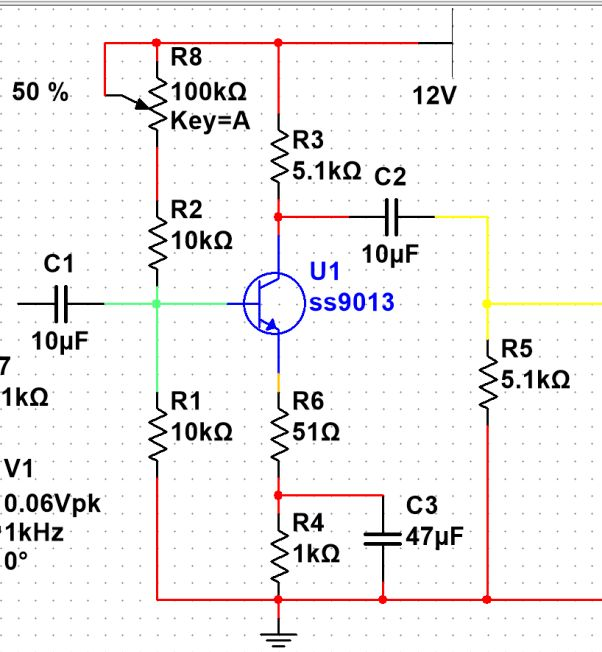
\includegraphics[width=0.72\textwidth]{figures/eda_sim/figure1.jpg}
    \caption{仿真电路原理图}
\end{figure}
\subsection*{8.1 静态工作点仿真}
\begin{figure}[H]
    \centering
    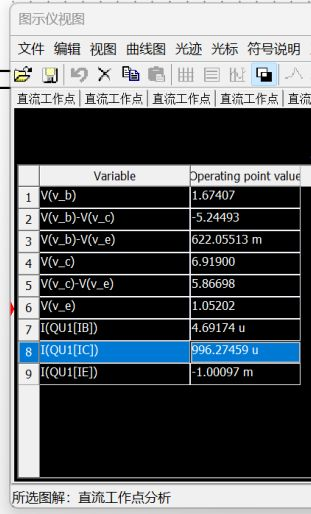
\includegraphics[width=0.72\textwidth]{figures/eda_sim/figure2.jpg}
    \caption{直流工作点分析结果}
\end{figure}
在Multisim中进行直流工作点分析，得到静态工作点参数如下表：
\begin{table}[H]
    \centering
    \begin{tabular}{|c|c|c|c|c|c|}
        \hline
        $V_{BQ}$ & $V_{EQ}$ & $V_{CQ}$ & $I_{BQ}$ &$ I_{CQ}$&$I_{EQ}$\\
        \hline
        1.67407\,V & 1.05202\,V & 6.91900\,V & 4.69174\,$\mu$A & 996.27459 \,$\mu$A & -1.00097\,$m$A \\
        \hline
    \end{tabular}
    \caption{静态工作点仿真结果}
\end{table}

与硬件实测结果对比可见：由于实际BJT和仿真模型参数存在差异，导致仿真结果与实测数据存在一定偏差，但总体趋势一致，均表明晶体管工作在放大区。

\subsection*{8.2 电压增益仿真}
\begin{figure}[H]
    \centering
    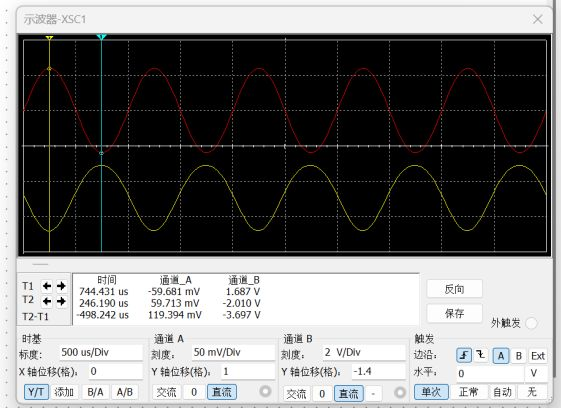
\includegraphics[width=0.72\textwidth]{figures/eda_sim/figure3.jpg}
    \caption{电压增益结果图}
\end{figure}
仿真得到电压增益
$$
A_v=\frac{V_o}{V_i} = \frac{3.679}{0.119} = 30.92.
$$
实测电压增益为
$$
A_v=34.81.
$$
两者相对误差约为 $ 11.2\%$，总体上较为接近，说明瞬态仿真与实测结果一致性较好，增益预测可靠。

\subsection*{8.3 通频带仿真}
\begin{figure}[H]
    \centering
    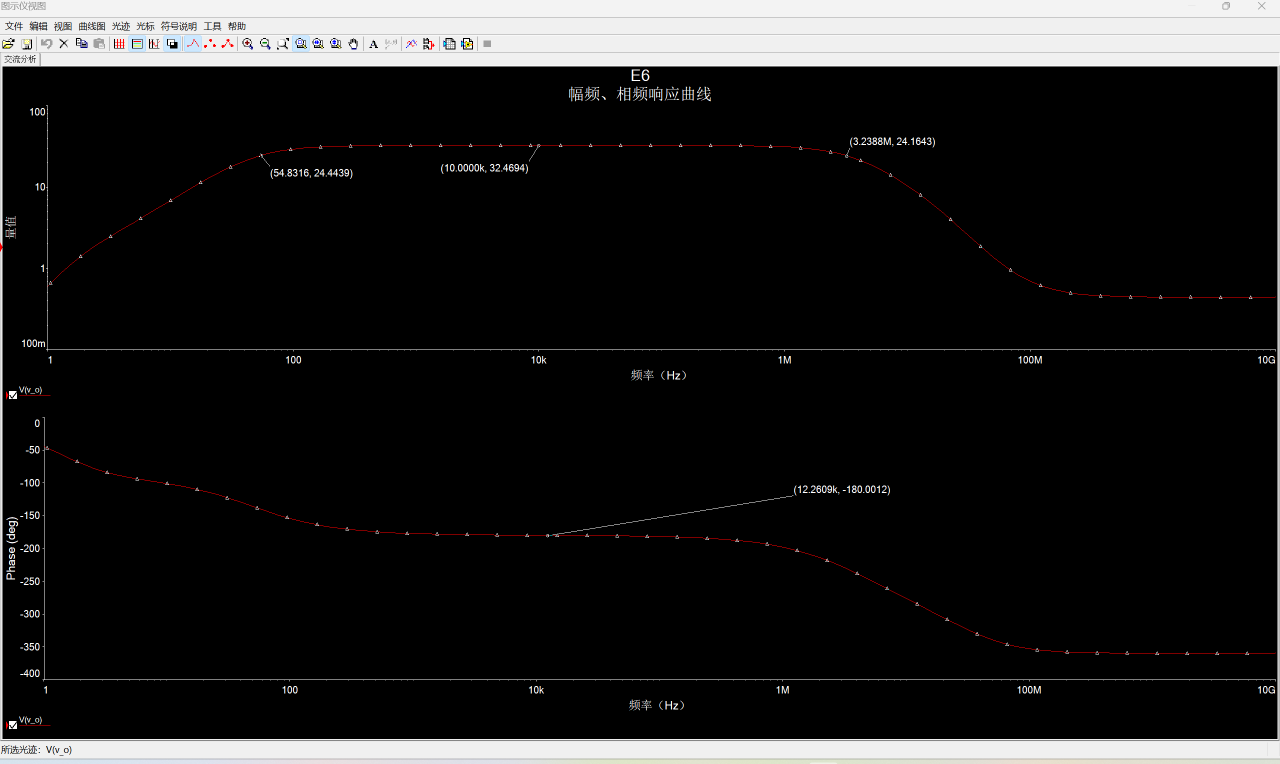
\includegraphics[width=0.72\textwidth]{figures/eda_sim/figure4.png}
    \caption{通频带分析结果图}
\end{figure}
仿真结果为：中频增益 $A_v=32.4696$($10kHz$)，下限频率 $f_L=54.8316\,\mathrm{Hz}$，上限频率
$f_H=3.2388\,\mathrm{MHz}$，通频带
$$
BW=f_H-f_L = 13.965\,\mathrm{MHz}.
$$

实测结果为：中频（$1\,\mathrm{kHz}$）增益 $34.07$，三分贝点增益 $24.62$，下限频率
$66.17\,\mathrm{Hz}$，上限频率 $870.39\,\mathrm{kHz}$，通频带约 $870.33\,\mathrm{kHz}$。

对比分析可知：下限频率与中频增益基本一致，但上限频率差异较大。主要原因是仿真中以SS9013代替实际使用的SS9018,其高频特性及参数仍与实际器件存在明显差异，该部分幅频响仿真仅可作定性参考。

\subsection*{8.4 输入电阻仿真}
\begin{figure}[H]
    \centering
    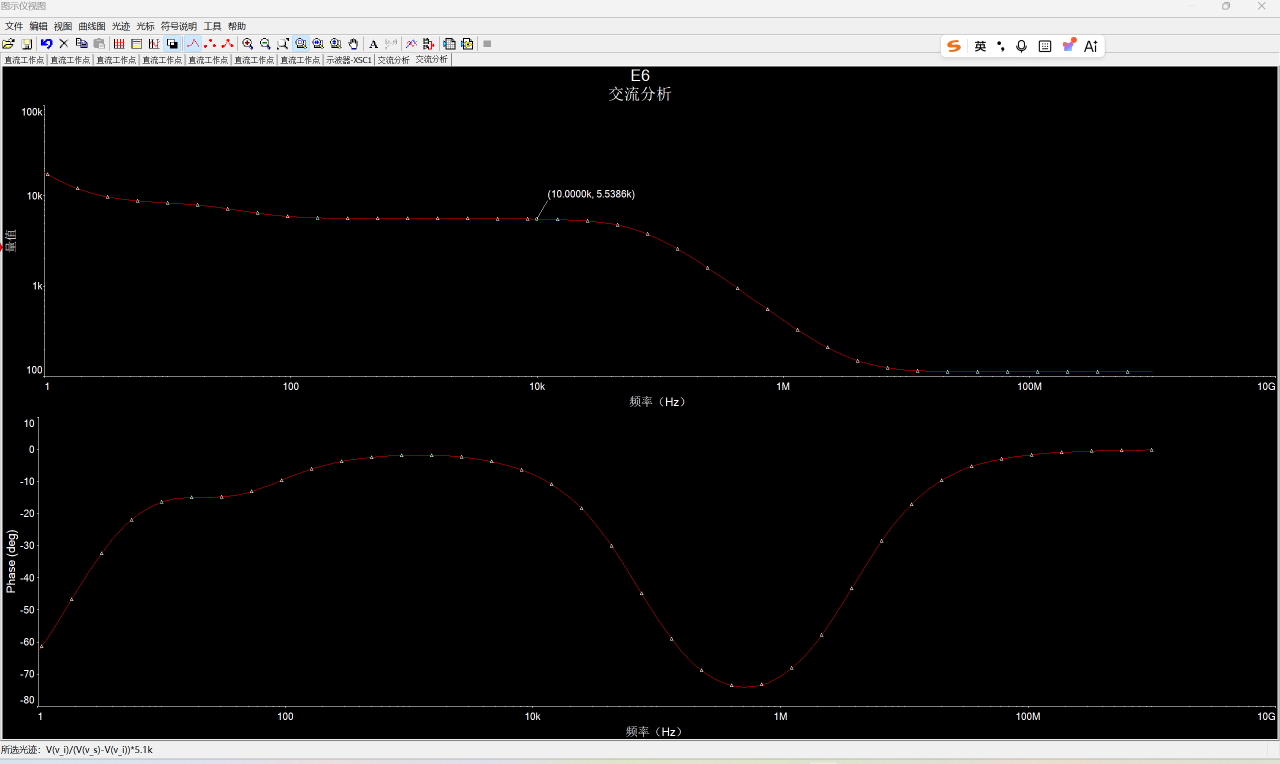
\includegraphics[width=0.72\textwidth]{figures/eda_sim/figure5.png}
    \caption{输入电阻分析结果图}
\end{figure}
仿真给出了输入电阻随频率变化的响应曲线。总体趋势为：低频段阻抗较大，随频率升高快速下降；进入中频段后趋于稳定；继续升频后再次下降。

从图中可以读出，在中频段仿真输入电阻约为 $5.5386\,\mathrm{k}\Omega$，而实测输入电阻约为 $4.29\,\mathrm{k}\Omega$，两者存在较大差异。主要原因是仿真中采用了替代三极管模型，导致输入电阻相关参数与实际器件存在较大偏差，因此仿真结果可信度有限，应以实测数据为主。

\subsection*{8.5 输出电阻仿真}
\begin{figure}[H]
    \centering
    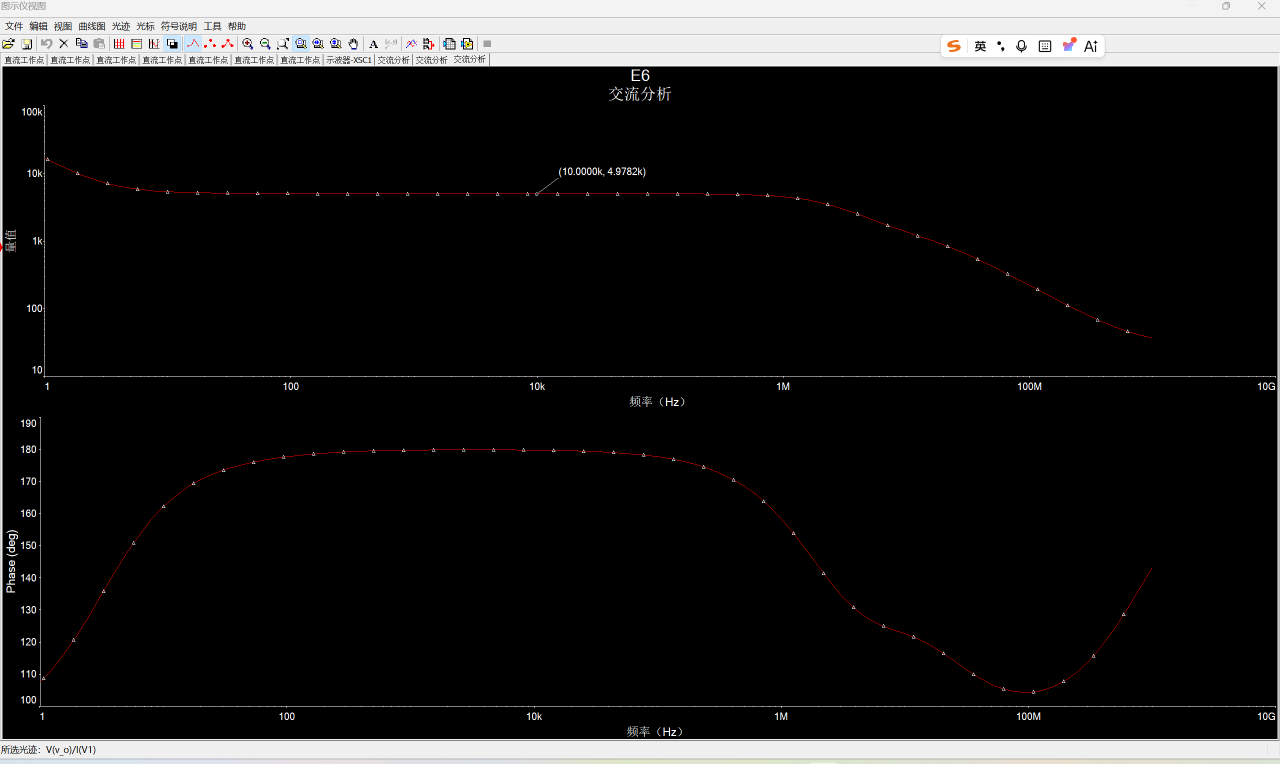
\includegraphics[width=0.72\textwidth]{figures/eda_sim/figure6.png}
    \caption{输出电阻分析结果图}
\end{figure}
仿真给出了输出电阻随频率变化的响应曲线。与输入电阻类似，总体趋势为：低频段阻抗较大，随频率升高快速下降；进入中频段后趋于稳定；继续升频后再次下降。

从图中可以读出，在中频段仿真输入电阻约为 $4.9782\,\mathrm{k}\Omega$，而实测输入电阻约为 $4.29\,\mathrm{k}\Omega$，两者较为接近。说明仿真模型在输出电阻预测方面较为可靠，且与实测结果一致性较好。

\section*{九、实验总结}
\subsection*{9.1 问题及解决方案}
\begin{enumerate}
    \item 测量增益时，发现波形总是出现截止失真的现象。排查发现主要原因为示波器误添加了直流偏置，调整示波器后测量结果正常。
    \item 测量通频带时，起初在升高和降低频率过程中观察到输出电压变化不明显，达到$100kHz$后仍未出现明显的增益下降，误以为电路异常。后续确认该放大电路通频带较宽，下限频率为几十赫兹，上限频率可达数兆赫兹，测试现象与电路特性一致。
    
\end{enumerate}

\subsection*{9.2 操作技巧}
\begin{enumerate}
    \item 电路搭建按标称值选取元件后，建议在数据计算前复测电阻、电容实际值，可有效减小器件公差累计带来的误差。
    \item 测试导线剥皮可采用“一端长、一端短”的方式：短端插入面包板更稳固，长端便于连接测试夹。应尽量避免“夹子互夹”，以降低接触不良概率并提高调试效率。
\end{enumerate}

\subsection*{9.3 心得体会}
通过本次实验，问题定位与排查能力得到进一步提升，面包板搭建与调试熟练度明显提高，同时也更加熟悉示波器在波形观察与参数测量中的使用方法。

\section*{十、思考题}
\begin{enumerate}
    \item 本实验若出现图示失真波形，试判断各属于哪种类型失真。

    \begin{center}
        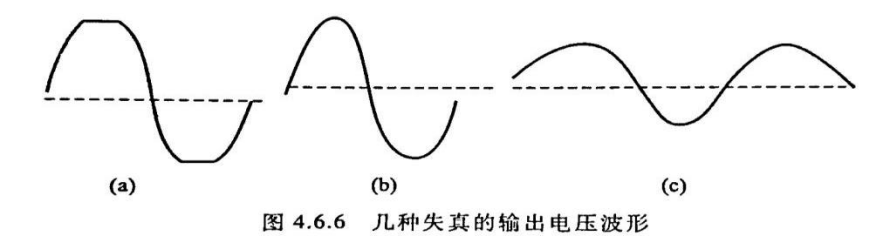
\includegraphics[width=0.62\textwidth]{thinking_problems/problem1.png}
    \end{center}

    \textbf{答：}a 图同时出现饱和失真与截止失真，属于非线性失真；b 图和 c 图均属于不对称失真。
    

    \item 测量放大器静态工作点时，若测得 $V_{CEQ}<0.5\,\mathrm{V}$，说明三极管处于什么工作状态？

    \textbf{答：}说明三极管已处于饱和状态。

    \item 当本实验电路出现饱和失真或截止失真时，应怎样调整电路参数以消除失真？

    
    \textbf{答：}若先出现饱和失真，说明静态工作点偏高，应增大电位器阻值，使静态工作点下移；若先出现截止失真，说明静态工作点偏低，应减小电位器阻值，使静态工作点上移。

    \item 负载电阻变化时，对放大电路静态工作点和电压增益分别有何影响？

    \textbf{答：}负载电阻变化对静态工作点影响较小（可近似认为无影响），但对电压增益影响较明显。

    \item 改变静态工作点时，对放大电路输入电阻有无影响？为什么？

    \textbf{答：}有一定影响。因为
    \[
    R_i=R_{B1}\parallel R_{B2}\parallel r_{be},\quad
    r_{be}\approx (1+\beta)\frac{26\,\mathrm{mV}}{I_E},
    \]
    当静态工作点升高时，$I_E$ 增大，$r_{be}$ 减小，从而 $R_i$ 也会相应减小。
\end{enumerate}

\end{document}